\chapter{自旋液体}\label{chap:spin-liquid}

大部分自旋系统(如\autoref{chap:magnetic}中展示的那些)在低温下都会落到铁磁序或反铁磁序中,因为零温时没有热涨落,而相互作用总是存在的,因此系统倾向于有序。
然而,如果零温时有特别强的量子涨落,可能系统基态中不存在这种类型的序,其中没有出现任何对称性自发破缺,无法定义序参量。
这样的自旋系统称为\concept{自旋液体},因为它们的基态是无序的,正如液体之于固体一样。
自旋液体的出现可能是因为在零温下由于一些阻挫(frustration, 即,让晶格取特定的形式使得反铁磁序无法形成)或者别的原因。
需注意自旋液体中没有对称性自发破缺,但是这并不代表自旋液体中没有其它类型的序和相变,例如,它们完全可以有拓扑序。
因此,自旋液体是一个非常有趣的状态,其制备方法以及性质都很引人注意。

虽然自旋液体似乎可以归结在磁性材料的范畴内,强烈的量子涨落实际上意味着自旋液体中有一些一般的磁性材料不会有的丰富行为。
在真正的自旋液体中我们会观察到演生规范场和拓扑序——实际上,自旋液体是除了分数量子霍尔效应以外仅有的已知的在实验上有可能实现的拓扑序。
分数量子霍尔效应确定有拓扑序,而目前没有确定无疑是自旋液体的材料,其它的拓扑序模型都是人为构造的。

\begin{figure}
    \centering
    \tikzset{every picture/.style={line width=0.75pt}} %set default line width to 0.75pt        

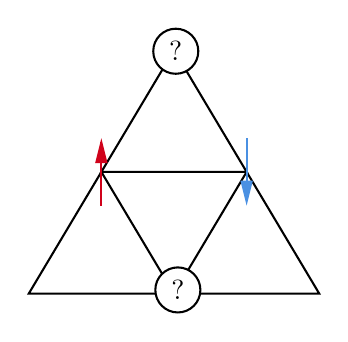
\begin{tikzpicture}[x=0.75pt,y=0.75pt,yscale=-1,xscale=1]
%uncomment if require: \path (0,300); %set diagram left start at 0, and has height of 300

%Shape: Triangle [id:dp3265971145624944] 
\draw   (225,126.33) -- (260,185) -- (190,185) -- cycle ;
%Shape: Triangle [id:dp457754747303309] 
\draw   (155,126.33) -- (190,185) -- (120,185) -- cycle ;
%Shape: Triangle [id:dp5282716496110524] 
\draw   (190,67.66) -- (225,126.33) -- (155,126.33) -- cycle ;
%Straight Lines [id:da7008008238341734] 
\draw [color={rgb, 255:red, 208; green, 2; blue, 27 }  ,draw opacity=1 ]   (155,142.56) -- (155,112.1) ;
\draw [shift={(155,110.1)}, rotate = 450] [fill={rgb, 255:red, 208; green, 2; blue, 27 }  ,fill opacity=1 ][line width=0.08]  [draw opacity=0] (12,-3) -- (0,0) -- (12,3) -- cycle    ;
%Straight Lines [id:da47122065737438956] 
\draw [color={rgb, 255:red, 74; green, 144; blue, 226 }  ,draw opacity=1 ]   (225,110.1) -- (225,140.56) ;
\draw [shift={(225,142.56)}, rotate = 270] [fill={rgb, 255:red, 74; green, 144; blue, 226 }  ,fill opacity=1 ][line width=0.08]  [draw opacity=0] (12,-3) -- (0,0) -- (12,3) -- cycle    ;
%Shape: Circle [id:dp2858034795038058] 
\draw  [fill={rgb, 255:red, 255; green, 255; blue, 255 }  ,fill opacity=1 ] (181,183.18) .. controls (181,177.19) and (185.86,172.33) .. (191.85,172.33) .. controls (197.85,172.33) and (202.71,177.19) .. (202.71,183.18) .. controls (202.71,189.18) and (197.85,194.04) .. (191.85,194.04) .. controls (185.86,194.04) and (181,189.18) .. (181,183.18) -- cycle ;

%Shape: Circle [id:dp48141040110301847] 
\draw  [fill={rgb, 255:red, 255; green, 255; blue, 255 }  ,fill opacity=1 ] (180,68.18) .. controls (180,62.19) and (184.86,57.33) .. (190.85,57.33) .. controls (196.85,57.33) and (201.71,62.19) .. (201.71,68.18) .. controls (201.71,74.18) and (196.85,79.04) .. (190.85,79.04) .. controls (184.86,79.04) and (180,74.18) .. (180,68.18) -- cycle ;


% Text Node
\draw (191.85,183.18) node   [align=left] {?};
% Text Node
\draw (190.85,68.18) node   [align=left] {?};


\end{tikzpicture}
    \caption{三角晶格上的阻挫:无法适当安排自旋方向让相邻自旋反向}
    \label{fig:triangular-frustration}
\end{figure}

\begin{info}{寻找自旋液体的尝试}{try-finding-spin-liquid}
    目前没有人找到确定无疑是自旋液体的材料。
    1973年,P.W.Anderson考虑了一个三角晶格上的反铁磁模型,来给反铁磁序的形成制造一些阻挫,因为三角晶格上显然无法形成反铁磁序(见\autoref{fig:triangular-frustration})。
    他猜测其基态为将晶格上最近邻自旋配对后将两个自旋自由度做分解
    \[
        \frac{1}{2} \otimes \frac{1}{2} = 0 \oplus 1,
    \]
    取所有可能的配对中的单态等权叠加的结果。这个状态称为\concept{RVB(Resonance Valence Bond)态}。
    如果实际上基态真的是RVB态,那么显然基态上没有形成任何磁性序,并且会有一些和磁性序上的“扰动”截然不同的激发(这些后文会详述)。
    事实证明这个说法是错误的:三角晶格上的海森堡模型的基态是一种特殊的铁磁态。虽然如此,自旋液体仍然是一个非常有趣的状态,因为,这可能是因为,对称性破缺不能发生。
    一些有机盐被认为有可能产生自旋液体,因为对它们做AMR实验观察不到任何磁性序,但始终没有定论;不少这种候选的自旋液体都被其它实验证实并非自旋液体了。
\end{info}

\section{各向同性海森堡模型演生出的自旋液体}

各向同性海森堡模型是
\begin{equation}
    H = J \sum_{\pair{\vb*{i}, \vb*{j}}} \vb*{S}_{\vb*{i}} \cdot \vb*{S}_{\vb*{j}}.
    \label{eq:heisenberg-model-spin-liquid}
\end{equation}
我们没有指定晶格是什么;本节将假定此模型在某个晶格上能够形成自旋液体,并且将处理自旋液体的标准手法作用于其上。

\subsection{三角晶格上的RVB态及其附近的低能激发}

\begin{back}{部分子构造}{parton-spin}
    \concept{部分子方法}是指将一个自旋自由度写成一些费米子或是玻色子自由度(即所谓\concept{部分子})的组合,自旋算符是两个费米子或是玻色子产生湮灭算符的乘积,然后施加适当的约束来保证拆分后的物理和拆分前相同。
    这相当于说,我们使用一个费米子系统或是玻色子系统实现了一个自旋系统。
    这种方法有时也称为\concept{投影构造}。
    这样做的好处在于,如果由此得到的费米子或玻色子理论中相互作用没有强到让这些费米子和玻色子又凝聚成对,那么实际上,这意味着自旋系统演生出了类似于费米子和玻色子的激发,即拆分得到的部分子正是自旋系统的低能自由度。

    只要算符的代数关系不变,并且将部分子系统的希尔伯特空间固定为每个格点上只有一个部分子的那部分,不同的拆分方式不会改变物理。
    对自旋系统,我们手动给不同格点上的自旋算符贴上位置标签,而对费米子/玻色子系统,坐标标签是粒子产生算符自带的参数,因此表面上看起来,拆分之后得到的费米子/玻色子系统的希尔伯特空间由于对称化/反对称化的要求而受到限制,似乎部分子系统的希尔伯特空间要比自旋系统的希尔伯特空间小,但是实际上两者是同构的:自旋系统的希尔伯特空间的基形如
    \[
        \ket{\sigma_1, \sigma_2, \ldots, \sigma_n}
    \]
    而部分子系统的希尔伯特空间的基形如
    \[
        {c}^\dagger_{1 \sigma_1} {c}^\dagger_{2 \sigma_2} \cdots {c}^\dagger_{n \sigma_n} \ket{0},
    \]
    后者中交换$1, 2$等空间标签,态矢量不变或者反号,所以两种系统的希尔伯特空间是一样大的。
    不施加费米统计或是玻色统计,粒子系统的希尔伯特空间实际上要比自旋系统的希尔伯特空间大,反倒是施加了对称/反对称要求之后两者是同构的。

    不过虽然部分子构造方式不改变物理,一些拆分方式中的部分子更加接近自旋系统中实际出现的激发,从而,使用这些拆分方法得到的部分子的理论使用平均场之类的方法处理得到的结果相比于其它方案是更加可靠的。
    这和\autoref{back:gl-hubbard-stratonovich}中选择序参量很相似。

    自旋系统演生出部分子这一事实是分数化现象的一种,即自旋系统中不同的“性质”(在这里是$1/2$自旋本身)似乎被不同的激发携带着。
\end{back}

\subsubsection{RVB态}

我们详细说明一下\autoref{info:try-finding-spin-liquid}中的RVB态。
所谓RVB态是指这样的基态:
\begin{equation}
    \ket*{\text{ground}} \propto \sum_{\text{all possible pair partitions}} \frac{1}{\sqrt{2}} (\ket*{\uparrow \downarrow} - \ket*{\downarrow \uparrow})_{\text{pair 1}} \otimes \frac{1}{\sqrt{2}} (\ket*{\uparrow \downarrow} - \ket*{\downarrow \uparrow})_{\text{pair 2}} \otimes \cdots, 
\end{equation}
即我们将三角晶格划分成许多不相交的相邻自旋对,然后让每个相邻自旋对上的两个自旋处于自旋单态,即$(\ket*{\uparrow \downarrow} - \ket*{\downarrow \uparrow}) / \sqrt{2}$上,将所有可能的这种态(\autoref{fig:rvb-component}展示了一个这样的态,其中被同一块黄色区域覆盖的两个格点上的自旋处在一个自旋单态中)等权叠加起来,就得到了一个RVB态。

\begin{figure}
    \centering
    \subfigure[RVB态中的一个成分]{
        

\tikzset{every picture/.style={line width=0.75pt}} %set default line width to 0.75pt        

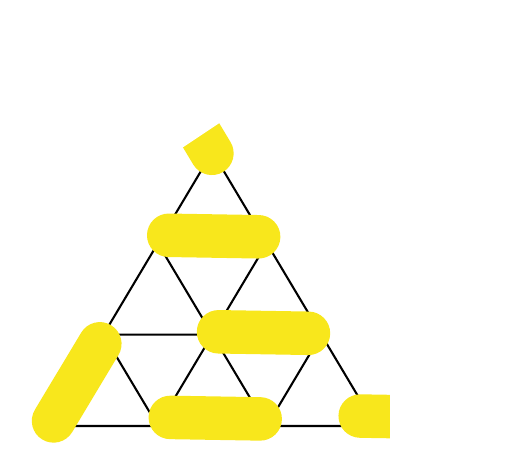
\begin{tikzpicture}[x=0.75pt,y=0.75pt,yscale=-0.75,xscale=0.75]
%uncomment if require: \path (0,300); %set diagram left start at 0, and has height of 300

%Shape: Triangle [id:dp5394198004259025] 
\draw   (272,182.33) -- (307,241) -- (237,241) -- cycle ;
%Shape: Triangle [id:dp0060243569953495335] 
\draw   (202,182.33) -- (237,241) -- (167,241) -- cycle ;
%Shape: Triangle [id:dp5009006316084215] 
\draw   (237,123.66) -- (272,182.33) -- (202,182.33) -- cycle ;
%Shape: Triangle [id:dp5954923975464252] 
\draw   (342,182.33) -- (377,241) -- (307,241) -- cycle ;
%Shape: Triangle [id:dp9717966554343387] 
\draw   (307,123.66) -- (342,182.33) -- (272,182.33) -- cycle ;
%Shape: Triangle [id:dp29175836331511373] 
\draw   (272,64.99) -- (307,123.66) -- (237,123.66) -- cycle ;
%Rounded Rect [id:dp9303927185789262] 
\draw  [draw opacity=0][fill={rgb, 255:red, 248; green, 231; blue, 28 }  ,fill opacity=1 ] (162.79,249.71) .. controls (156.17,245.74) and (154.03,237.15) .. (158,230.54) -- (187.75,181.02) .. controls (191.72,174.4) and (200.3,172.26) .. (206.92,176.24) -- (206.92,176.24) .. controls (213.53,180.21) and (215.67,188.79) .. (211.7,195.41) -- (181.96,244.92) .. controls (177.99,251.54) and (169.4,253.68) .. (162.79,249.71) -- cycle ;
%Rounded Rect [id:dp2973774835771079] 
\draw  [draw opacity=0][fill={rgb, 255:red, 248; green, 231; blue, 28 }  ,fill opacity=1 ] (230.01,118.26) .. controls (230.13,110.55) and (236.49,104.4) .. (244.21,104.52) -- (301.96,105.48) .. controls (309.68,105.61) and (315.83,111.97) .. (315.7,119.68) -- (315.7,119.68) .. controls (315.57,127.4) and (309.21,133.55) .. (301.5,133.42) -- (243.74,132.46) .. controls (236.03,132.34) and (229.88,125.98) .. (230.01,118.26) -- cycle ;
%Rounded Rect [id:dp7712557322954827] 
\draw  [draw opacity=0][fill={rgb, 255:red, 248; green, 231; blue, 28 }  ,fill opacity=1 ] (231.01,235.26) .. controls (231.13,227.55) and (237.49,221.4) .. (245.21,221.52) -- (302.96,222.48) .. controls (310.68,222.61) and (316.83,228.97) .. (316.7,236.68) -- (316.7,236.68) .. controls (316.57,244.4) and (310.21,250.55) .. (302.5,250.42) -- (244.74,249.46) .. controls (237.03,249.34) and (230.88,242.98) .. (231.01,235.26) -- cycle ;
%Rounded Rect [id:dp25009751823087134] 
\draw  [draw opacity=0][fill={rgb, 255:red, 248; green, 231; blue, 28 }  ,fill opacity=1 ] (262.01,180.26) .. controls (262.13,172.55) and (268.49,166.4) .. (276.21,166.52) -- (333.96,167.48) .. controls (341.68,167.61) and (347.83,173.97) .. (347.7,181.68) -- (347.7,181.68) .. controls (347.57,189.4) and (341.21,195.55) .. (333.5,195.42) -- (275.74,194.46) .. controls (268.03,194.34) and (261.88,187.98) .. (262.01,180.26) -- cycle ;
%Rounded Rect [id:dp12607246135910644] 
\draw  [draw opacity=0][fill={rgb, 255:red, 248; green, 231; blue, 28 }  ,fill opacity=1 ] (353.01,234.39) .. controls (353.13,226.67) and (359.49,220.52) .. (367.21,220.65) -- (424.96,221.61) .. controls (432.68,221.73) and (438.83,228.09) .. (438.7,235.81) -- (438.7,235.81) .. controls (438.57,243.52) and (432.21,249.67) .. (424.5,249.55) -- (366.74,248.59) .. controls (359.03,248.46) and (352.88,242.1) .. (353.01,234.39) -- cycle ;
%Shape: Rectangle [id:dp4625096290080499] 
\draw  [draw opacity=0][fill={rgb, 255:red, 255; green, 255; blue, 255 }  ,fill opacity=1 ] (386,214) -- (450.71,214) -- (450.71,254) -- (386,254) -- cycle ;
%Rounded Rect [id:dp22383160699593008] 
\draw  [draw opacity=0][fill={rgb, 255:red, 248; green, 231; blue, 28 }  ,fill opacity=1 ] (234.81,4.31) .. controls (241.43,0.34) and (250.01,2.49) .. (253.98,9.11) -- (283.69,58.65) .. controls (287.66,65.26) and (285.51,73.85) .. (278.89,77.81) -- (278.89,77.81) .. controls (272.27,81.78) and (263.69,79.64) .. (259.72,73.02) -- (230.02,23.48) .. controls (226.05,16.86) and (228.2,8.28) .. (234.81,4.31) -- cycle ;
%Shape: Rectangle [id:dp768095676065814] 
\draw  [draw opacity=0][fill={rgb, 255:red, 255; green, 255; blue, 255 }  ,fill opacity=1 ] (246.79,66.21) -- (207.94,7.98) -- (241.21,-14.21) -- (280.06,44.02) -- cycle ;




\end{tikzpicture}

        \label{fig:rvb-component}
    }
    \subfigure[一种低能激发态:一个自旋单态“对”被解开,产生两个向上的自旋]{
        

\tikzset{every picture/.style={line width=0.75pt}} %set default line width to 0.75pt        

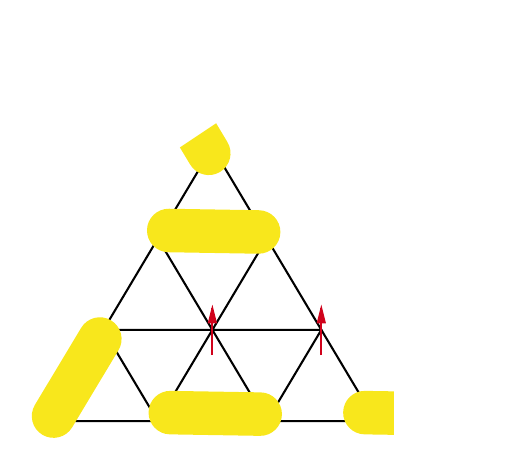
\begin{tikzpicture}[x=0.75pt,y=0.75pt,yscale=-0.75,xscale=0.75]
%uncomment if require: \path (0,300); %set diagram left start at 0, and has height of 300

%Shape: Triangle [id:dp7709012666212918] 
\draw   (292,174.46) -- (327,233.12) -- (257,233.12) -- cycle ;
%Shape: Triangle [id:dp9295040886868511] 
\draw   (222,174.46) -- (257,233.12) -- (187,233.12) -- cycle ;
%Shape: Triangle [id:dp177949788580418] 
\draw   (257,115.79) -- (292,174.46) -- (222,174.46) -- cycle ;
%Shape: Triangle [id:dp03247866415223255] 
\draw   (362,174.46) -- (397,233.12) -- (327,233.12) -- cycle ;
%Shape: Triangle [id:dp26037578632796765] 
\draw   (327,115.79) -- (362,174.46) -- (292,174.46) -- cycle ;
%Shape: Triangle [id:dp3012062348071127] 
\draw   (292,57.12) -- (327,115.79) -- (257,115.79) -- cycle ;
%Rounded Rect [id:dp4030558357818268] 
\draw  [draw opacity=0][fill={rgb, 255:red, 248; green, 231; blue, 28 }  ,fill opacity=1 ] (182.79,241.83) .. controls (176.17,237.86) and (174.03,229.28) .. (178,222.66) -- (207.75,173.14) .. controls (211.72,166.53) and (220.3,164.39) .. (226.92,168.36) -- (226.92,168.36) .. controls (233.53,172.33) and (235.67,180.92) .. (231.7,187.53) -- (201.96,237.05) .. controls (197.99,243.66) and (189.4,245.81) .. (182.79,241.83) -- cycle ;
%Rounded Rect [id:dp16737425370308645] 
\draw  [draw opacity=0][fill={rgb, 255:red, 248; green, 231; blue, 28 }  ,fill opacity=1 ] (250.01,110.39) .. controls (250.13,102.67) and (256.49,96.52) .. (264.21,96.65) -- (321.96,97.61) .. controls (329.68,97.73) and (335.83,104.09) .. (335.7,111.81) -- (335.7,111.81) .. controls (335.57,119.52) and (329.21,125.67) .. (321.5,125.55) -- (263.74,124.59) .. controls (256.03,124.46) and (249.88,118.1) .. (250.01,110.39) -- cycle ;
%Rounded Rect [id:dp7997977143532831] 
\draw  [draw opacity=0][fill={rgb, 255:red, 248; green, 231; blue, 28 }  ,fill opacity=1 ] (251.01,227.39) .. controls (251.13,219.67) and (257.49,213.52) .. (265.21,213.65) -- (322.96,214.61) .. controls (330.68,214.73) and (336.83,221.09) .. (336.7,228.81) -- (336.7,228.81) .. controls (336.57,236.52) and (330.21,242.67) .. (322.5,242.55) -- (264.74,241.59) .. controls (257.03,241.46) and (250.88,235.1) .. (251.01,227.39) -- cycle ;
%Straight Lines [id:da8204619655647556] 
\draw [color={rgb, 255:red, 208; green, 2; blue, 27 }  ,draw opacity=1 ]   (292,190.68) -- (292,160.23) ;
\draw [shift={(292,158.23)}, rotate = 450] [fill={rgb, 255:red, 208; green, 2; blue, 27 }  ,fill opacity=1 ][line width=0.08]  [draw opacity=0] (12,-3) -- (0,0) -- (12,3) -- cycle    ;
%Straight Lines [id:da301443667677862] 
\draw [color={rgb, 255:red, 208; green, 2; blue, 27 }  ,draw opacity=1 ]   (362,190.68) -- (362,160.23) ;
\draw [shift={(362,158.23)}, rotate = 450] [fill={rgb, 255:red, 208; green, 2; blue, 27 }  ,fill opacity=1 ][line width=0.08]  [draw opacity=0] (12,-3) -- (0,0) -- (12,3) -- cycle    ;
%Rounded Rect [id:dp28390331250432066] 
\draw  [draw opacity=0][fill={rgb, 255:red, 248; green, 231; blue, 28 }  ,fill opacity=1 ] (376.01,227.39) .. controls (376.13,219.67) and (382.49,213.52) .. (390.21,213.65) -- (447.96,214.61) .. controls (455.68,214.73) and (461.83,221.09) .. (461.7,228.81) -- (461.7,228.81) .. controls (461.57,236.52) and (455.21,242.67) .. (447.5,242.55) -- (389.74,241.59) .. controls (382.03,241.46) and (375.88,235.1) .. (376.01,227.39) -- cycle ;
%Shape: Rectangle [id:dp4527570591753749] 
\draw  [draw opacity=0][fill={rgb, 255:red, 255; green, 255; blue, 255 }  ,fill opacity=1 ] (409,207) -- (473.71,207) -- (473.71,247) -- (409,247) -- cycle ;
%Rounded Rect [id:dp3963770711962662] 
\draw  [draw opacity=0][fill={rgb, 255:red, 248; green, 231; blue, 28 }  ,fill opacity=1 ] (252.81,-0.47) .. controls (259.43,-4.44) and (268.01,-2.29) .. (271.98,4.32) -- (301.69,53.86) .. controls (305.66,60.48) and (303.51,69.06) .. (296.89,73.03) -- (296.89,73.03) .. controls (290.27,77) and (281.69,74.85) .. (277.72,68.23) -- (248.02,18.69) .. controls (244.05,12.08) and (246.2,3.49) .. (252.81,-0.47) -- cycle ;
%Shape: Rectangle [id:dp5531026767203489] 
\draw  [draw opacity=0][fill={rgb, 255:red, 255; green, 255; blue, 255 }  ,fill opacity=1 ] (264.79,61.43) -- (225.94,3.2) -- (259.21,-19) -- (298.06,39.23) -- cycle ;




\end{tikzpicture}

        \label{fig:rvb-up-excitation}
    }
    \caption{RVB态及其元激发}
\end{figure}

现在我们分析RVB态之上的元激发。将相邻的两个自旋当成一个自由度,则它可以分解为
\begin{equation}
    \frac{1}{2} \otimes \frac{1}{2} = 0 \oplus 1,
\end{equation}
RVB态中,像\autoref{fig:rvb-component}中这样被同一块黄色区域覆盖的两个格点占据上式中的单态,那么可以给系统一个局域的激励,让某一对最近邻格点的状态变成一个自旋三重态。
\autoref{fig:rvb-up-excitation}展示了一种这样的激发态:一个$(\ket*{\uparrow \downarrow} - \ket*{\downarrow \uparrow}) / \sqrt{2}$态被激发成$\ket*{\uparrow \uparrow}$,图形化地展示就是。
组成自旋三态的两个自旋可以跑:我们总是可以重新安排自旋配对,于是我们可以认为自旋$1$的激发被拆成了两半,每一个都可以四处移动。这就得到了\concept{自旋子(spinon)}。
可以验证这是费米子,
这些自旋子全部都是自旋$1/2$的,并且总是有偶数个自旋子。

因此,至少有一类自旋系统——基态为RVB态的自旋液体——中可以演生出费米子激发,这让我们有理由相信,做费米型的部分子拆分至少对一些自旋系统是合理的。

\subsubsection{slave boson方法}

我们对海森堡模型使用\concept{slave boson}方法,这是指做分解
\begin{equation}
    {S}_{\vb*{i}} = \frac{1}{2} {f}_{\vb*{i} \alpha}^\dagger \vb*{\sigma}_{\alpha \beta} f_{\vb*{i} \beta},
\end{equation}
其中${f}$为费米子;每个格点上的自旋的取值由这个格点上的费米型部分子的自旋携带。
这个方法本来是用于分析携带电荷的费米子的,但是后来被用在了分析自旋上,相应的这种方法分解出来的部分子在自旋系统中就是费米子而不是玻色子。
使用费米型部分子的好处在于可以避免玻色子陷入玻色-爱因斯坦凝聚态;如果自旋系统中的元激发实际上并不处在玻色-爱因斯坦凝聚态,这就意味着我们需要某种很强的玻色型部分子之间的相互作用让玻色-爱因斯坦凝聚态不稳定,即需要很强的量子涨落,于是我们无非是把一个强关联问题转化成了另一个强关联问题。
但是,如前所述,RVB态附近的激发真的好像一个费米子,所以我们有理由相信,如果在某个晶格上海森堡模型\eqref{eq:heisenberg-model-spin-liquid}真的演生出了基态是RVB态的自旋液体,那么slave boson构造就是合理的。

\subsection{费米子哈密顿量和演生$U(1)$规范场}

\subsubsection{受约束的费米子哈密顿量}

做了slave boson分解之后,哈密顿量就成为一个四阶项,描述了两个费米子的散射,写出来是
\[
    {H} = \frac{J}{4} \sum_{\pair{\vb*{i}, \vb*{j}}} (2 {f}^\dagger_{\vb*{i} \alpha} {f}_{\vb*{i} \beta} {f}_{\vb*{j} \beta}^\dagger {f}_{\vb*{j} \alpha} - {f}^\dagger_{\vb*{i} \alpha} {f}_{\vb*{i} \alpha} {f}^\dagger_{\vb*{j} \beta} {f}_{\vb*{j} \beta}),
\]
第二项由于我们要求每个格点只有单占据而可以略去,于是
\begin{equation}
    {H} = - \frac{J}{2} \sum_{\pair{\vb*{i}, \vb*{j}}} {f}_{\vb*{i} \alpha}^\dagger {f}_{\vb*{j} \beta}^\dagger {f}_{\vb*{i} \beta} {f}_{\vb*{j} \alpha}.
    \label{eq:slave-boson-hamiltonian}
\end{equation}
这个哈密顿量所在的希尔伯特空间是每个格点上有且只有一个费米子的这部分空间,写成公式就是
\begin{equation}
    f_{\vb*{i} \alpha}^\dagger f_{\vb*{j} \alpha} = 1, 
    \label{eq:one-site-one-fermion}
\end{equation}
注意其中$\vb*{i}$不求和而$\alpha$求和。
这个约束在接下来的计算中必须始终被考虑到,它的一个直接推论是
\begin{equation}
    \epsilon_{\alpha \beta} f_{\vb*{i} \alpha} f_{\vb*{i} \beta} = 0.
\end{equation}
\eqref{eq:slave-boson-hamiltonian}本身不会将一个满足\eqref{eq:one-site-one-fermion}的态转化成一个不满足这一限制的态,因此这里没有任何矛盾。

\subsubsection{路径积分和演生规范场}

下面我们使用路径积分方法引入约束\eqref{eq:one-site-one-fermion}。使用一个逐点的拉格朗日乘子$\lambda$来施加约束条件,我们有
\begin{equation}
    S[f, \bar{f}, \lambda] = \int_0^\beta \dd{\tau} \left( \sum_{\vb*{i}} \bar{f}_{\vb*{i} \alpha} \partial_\tau f_{\vb*{i} \alpha} + \sum_{\vb*{i}} \ii \lambda_{\vb*{i}} (\bar{f}_{\vb*{i} \alpha} f_{\vb*{i} \alpha} - 1) - \frac{J}{2} \sum_{\pair{\vb*{i}, \vb*{j}}} \bar{f}_{\vb*{i} \alpha} \bar{f}_{\vb*{j} \beta} f_{\vb*{j} \alpha} f_{\vb*{i} \beta} \right).
    \label{eq:spin-liquid-action}
\end{equation}
积掉拉格朗日乘子$\lambda_{\vb*{i}}$就能产生硬约束\eqref{eq:one-site-one-fermion}。

我们注意到,$\lambda_{\vb*{i}}$出现的位置和电势基本上一模一样(见\eqref{eq:imaginary-em-covariant-derivative}),且显然具有局域$U(1)$对称性。
这让我们猜测,\eqref{eq:spin-liquid-action}实际是一个自旋$1/2$费米子和某个$U(1)$规范场耦合的理论。
实际上,容易验证,将理论
\begin{equation}
    S[f, \bar{f}, \lambda, \chi, \bar{\chi}] = \int_0^\beta \dd{\tau} \left( \sum_{\vb*{i}} \bar{f}_{\vb*{i} \alpha} \partial_\tau f_{\vb*{i} \alpha} + \sum_{\vb*{i}} \ii \lambda_{\vb*{i}} (\bar{f}_{\vb*{i} \alpha} f_{\vb*{i} \alpha} - 1) + \frac{J}{2} \sum_{\pair{\vb*{i}, \vb*{j}}} (\abs{\chi_{\vb*{i} \vb*{j}}}^2 - \chi_{\vb*{i} \vb*{j}} \bar{f}_{\vb*{i} \alpha} f_{\vb*{j} \alpha} + \text{h.c.}) \right)
\end{equation}
积掉$\chi$,得到的正是\eqref{eq:spin-liquid-action}。
上式对应的哈密顿量是(注意)
\begin{equation}
    H = 
\end{equation}

如果\eqref{eq:spin-liquid-action}有非平庸的鞍点解,它附近的涨落肯定会破坏一些局域$U(1)$对称性。
现在我们假定在某些情况下可以有这样的鞍点解:$\Delta_{\vb*{i} \vb*{j}}$非零,但是$\chi_{\vb*{i} \vb*{j}}$为零。
此时
\begin{equation}
    S = \int_0^\beta \dd{\tau} \left( \sum_{\vb*{i}} \bar{f}_{\vb*{i} \alpha} (\partial_\tau - \ii \lambda_{\vb*{i}}) f_{\vb*{i} \alpha} - \tilde{J} \sum_{\pair{\vb*{i}, \vb*{j}}} \bar{\Delta}_{\vb*{i} \vb*{j}} \epsilon_{\alpha \beta} b_{\vb*{i} \alpha} b_{\vb*{j} \beta} + \text{h.c.} \right)
\end{equation}

\subsection{格点$U(1)$规范场论}

\subsubsection{平均场方法}

设
\begin{equation}
    {\Delta}_{\vb*{i} \vb*{j}} = \epsilon_{\alpha \beta} {f}_{\vb*{i} \alpha} {f}_{\vb*{j} \beta}, \quad {\chi} = {f}^\dagger_{\vb*{i} \alpha} {f}_{\vb*{j} \alpha},
\end{equation}
有
\begin{equation}
    {H} = - \frac{J}{2} \sum_{\pair{\vb*{i}, \vb*{j}}} {\Delta}^\dagger_{\vb*{i} \vb*{j}} {\Delta}_{\vb*{i} \vb*{j}} = - \frac{J}{2} \sum_{\pair{\vb*{i}, \vb*{j}}} {\chi}_{\vb*{i} \vb*{j}}^\dagger {\chi}_{\vb*{i} \vb*{j}} = - \frac{J}{4} \sum_{\pair{\vb*{i}, \vb*{j}}} ({\Delta}^\dagger_{\vb*{i} \vb*{j}} {\Delta}_{\vb*{i} \vb*{j}} + {\chi}^\dagger_{\vb*{i} \vb*{j}} {\chi}_{\vb*{i} \vb*{j}}),
\end{equation}
于是可以对最后一个形式做平均场近似;我们引入了两个参量,为了增加变分计算的参数,使之更加有效。
直接做平均场分解,有(我们将算符的期望值去掉帽子)
\[
    {H}_\text{MF} = - \frac{J}{4} \sum_{\pair{\vb*{i}, \vb*{j}}} (\Delta_{\vb*{i} \vb*{j}}^* {\Delta}_{\vb*{i} \vb*{j}} + {\Delta}_{\vb*{i} \vb*{j}} \Delta_{\vb*{i} \vb*{j}} - \abs*{\Delta_{\vb*{i} \vb*{j}}}^2) - \frac{J}{4} \sum_{\pair{\vb*{i}, \vb*{j}}} (\chi_{\vb*{i} \vb*{j}}^* {\chi}_{\vb*{i} \vb*{j}} + {\chi}_{\vb*{i} \vb*{j}} \chi_{\vb*{i} \vb*{j}} - \abs*{\chi_{\vb*{i} \vb*{j}}}^2).
\]
但是,实际上应该将系数设置成$3/8$,因为数值计算说明,直接做平均场近似效果非常糟糕。我们下面将会将系数统一称为$\tilde{J}$。
实际上严格计算平均场理论并没有什么意义,因为平均场理论的定量结果向来是非常糟糕的,而使用变分蒙特卡洛方法不难得到较为精确的结果。

原则上我们可以从平均场理论出发,通过一些方法——如大$N$展开,这里$N=2$——计算更高阶修正,但是这样非常繁琐,而仅计算有限阶可能效果也不好。

我们很关心演生规范场是不是禁闭的,如果是的话,它将不会有任何物理效应,因为低能下不会出现任何规范场涨落,而如果能量足够高,那就不再能够“只考虑基态附近的涨落”。

在格点规范场中允许存在磁单极子;此时它称为\concept{紧致的规范场},因为规范群是紧致的。
实际上,电动力学在格点上的规范群并不是$U(1)$的,因为$0$和$2\pi$不等价。

还有一种拆分方式:slave fermion,即Schwinger boson

参考: RMP 78 17 2006

\subsection{元激发和拓扑序}

举例:Resonance Valence Bond state : superposition of all pairing configurations, not a product state
看到一个

spin singlet pairs

但是,这就得到了spinon
有$\mathbb{Z}_2$-charge, so there are $\mathbb{Z}_2$-vortices.

TODO:为什么能够认为

Since $e$ and $m$ determines remaining states

spinon must carry a half-integer spin, and odd  of spoinons 

flux-fusion anomaly test

vison带有整数自旋(由于只区分拓扑性质,可以认为vison不带自旋,因为带有自旋的vison可以分解成一个带有自旋的平凡的激发和一个不带有自旋的vison激发)

Insertion of 

LSM theorem: if in each unit cell of a system there are odd spin-$1/2$, there must be ground state degeneracy.

possible phases:

\begin{enumerate}
    \item Trivial paramagnet: no ground state degeneracy
    \item Symmetry-breaking phases: FM, AFM, VBS, etc. Ground state degeneracy due to symmetry breaking.
    \item GSD on a torus, due to topological order
    \item GSD due to gapless excitations / 
\end{enumerate}

The theorem and the boundary of a topological state look quite alike, and this is not coincidence.

spin-1/2 edge of a spin AKLT chain

\subsection{演生规范场}

严格来说,此时做平均场是有问题的,因为我们手动地破缺了每个格点上粒子数始终唯一的限制,但是实际上,由于这个费米子模型实际上是一个自旋模型,这样的破缺是不正确的。
为此需要加入一个拉格朗日乘子项来固定每个格点上的粒子数,具体的拉格朗日乘子大小不能确定,是路径积分中需要额外做积分的一个场变量。

总之,在做平均场近似时我们得到了一个演生的规范场。

RMP 51, 657, 1979

总之,我们到现在用到了这些激发:我们观察到自旋液体系统中会有玻色spinon激发,这启发我们将自旋自由度拆分成玻色子,期望能够得到一个关于spinon激发的有效理论。
对拆分完成后的哈密顿量做约束以要求格点上玻色子单占据,并作平均场理论,我们得到一个规范场理论,拆分出的玻色子是物质场,还有一个定义在格子的边上的规范联络。
我们分析这个演生规范场,积掉spinon激发(实际上是自旋自由度拆分出的玻色子,我们相信它具有spinon的意义),得到一个纯粹的规范场理论(其中有动力学未给定的规范荷,可以据此定性分析spinon和规范场的相互作用),并发现这个规范场理论对应一个横场伊辛模型,它的铁磁相对应一个禁闭相,其中

\subsection{自旋液体中的对称性分数化}

大部分对称性都有所谓的对称性反常,需要生存在高维SPT(??)的边界态上。
直接从对称性分析出发可以得到大量的态,但是满足一定非常合理的条件的态是很少的,这些态均可以直接使用平均场构造出来。

Tensor category group cohomology(??)

边界和bulk上中的态都